\documentclass[a4paper,12pt]{article} % тип документа
\usepackage[margin=1in]{geometry} % Поля

%  Русский язык
\usepackage[warn]{mathtext}
\usepackage[T2A]{fontenc}			% кодировка
\usepackage[utf8]{inputenc}			% кодировка исходного текста
\usepackage[english,russian]{babel}	% локализация и переносы
% Математика
\usepackage{amsmath,amsfonts,amssymb,amsthm,mathtools} 
\usepackage{wasysym}
%%%
\usepackage{graphicx}

\usepackage{tabularx}

\usepackage{gensymb} % знак градуса
\usepackage{enumitem} % изменить список enumerate
\usepackage{placeins} % \FloatBarrier

\renewcommand{\thesection}{\Roman{section}} 
\renewcommand{\thesubsection}{\roman{subsection}}


\begin{document}

\newcolumntype{Y}{>{\centering\arraybackslash}X} %new tabularx


%титул
\hrule 	
\medskip
\begin{raggedright}
{\large \textbf{Отчёт по работе 3.4.1}}
\\
\medskip
{\Large Диа- и парамагнетики} 
\\
\medskip
{\large Карташов Констанин Б04-005}
\medskip
\hrule
\medskip
\end{raggedright}


\section{Анотация}

\paragraph{Цель работы:} 
Измерение магнитной восприимчивости диа- и параметрических образцов.

\paragraph{Оборудование:}
\begin{itemize}
\renewcommand{\labelitemi}{$\triangleright$}
\itemsep0em
\item электромагнит,
\item весы,
\item милливеберметр,
\item источник постоянного тока,
\item образцы диа- и парамагнетика.
\end{itemize}


\medskip\hrule\medskip

\section{Теоретическая часть}

\subsection{Краткие теоретические сведения}

\paragraph{Магнитная восприимчивость} тела может быть определена измерением сил, действующих на это тело в магнитном поле. Существуют два классических метода таких измерений: метод \textit{Фарадея }и метод \textit{Гюи}. В методе Гюи используется тонкий и длинный стержень, один из концов которого помещают в зазор электромагнита (в область однородного поля), а другой конец -- вне зазора, где величиной магнитного поля можно пренебречь. Тогда сила, действующая на помещённый образец равна:

\[
F_m = \left( \frac{\partial W_m}{\partial x} \right) \approx \chi \frac{B_0^2}{2 \mu_0} S.
\]

Знак силы зависит от восприимчивости $\chi$: парамагнетики $(\chi > 0)$ втягиваются в зазор электромагнита, а диамагнетики $(\chi < 0)$ выталкиваются из него. Таким образов рассчитав силу действующую на образец в известном магнитном поле, можно рассчитать его магнитную восприимчивость.

\subsection{Описание экспериментальной установки}

Схема установки приведена на рис. \ref{fig:setup}. Она состоит из:
\textbf{Электромагнита} с зазором. Поле в зазоре можно считать практически однородным
так как размеры полюсов значительно превышают размер зазора. 
\textbf{Источника питания} с регулируемым постоянным током. Величина тока задаётся при
помощи амперметра. Дли градуировки электромагнита используется \textbf{милливеберметр}.
\textbf{Весов} на которые подвешивается образец.

\FloatBarrier

\begin{figure}
\begin{center}
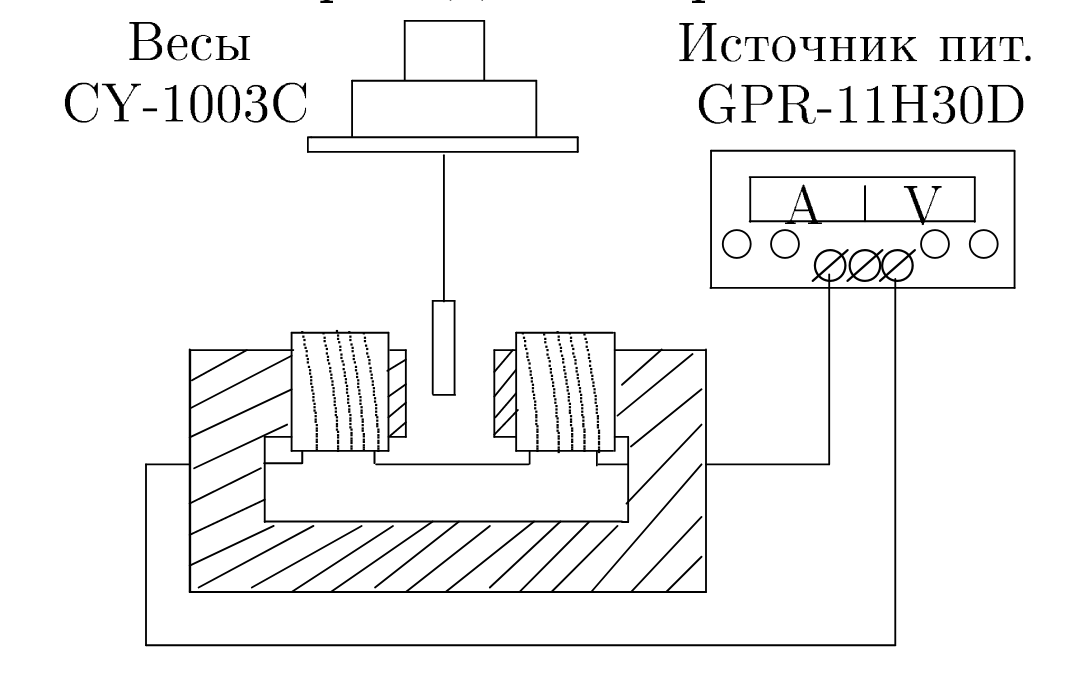
\includegraphics[width=0.5\linewidth]{setup.png}
\caption{Схема экспериментальной установки}
\label{fig:setup}
\end{center}
\end{figure}

\medskip\hrule\medskip

\section{Экспериментальная часть}

\subsection{Построение градуировочной прямой для электромагнита}

\textbf{Измерим} индукцию магнитного поля в зазоре пользуясь милливеберметром, пользуясь 
формулой $B = \Phi / S_n$. Значение $S_n = 72$ см$^2$. Измерим поток $\Phi$ между полюсами
при различных значениях тока на обмотке электромагнита, и посчитаем индукцию. Результаты измерений предствалены в таблице \ref{tab:grad}, на основании который построен график \ref{fig:grad_plot}. Погрешность измерения силы тока $\Delta I = 0.01$ А, погрешность милливеберметра $\Delta \Phi = 0.05$ мВб, и следовательно погрешность измерения $\Delta B = \Delta \Phi / S_n = 7$ мТл.

\begin{table}[h]
\begin{center}
\begin{tabular}{|c|c|c|c|c|c|c|c|c|}
\hline 
$I$, А & 0.3 & 0.7 & 1.1 & 1.5 & 1.9 & 2.3 & 2.6 & 3.0 \\ 
\hline 
$\Phi$, мВб & 0.4 & 1.3 & 2.7 & 3.6 & 4.5 & 5.4 & 6 & 6.7 \\ 
\hline 
$B$, мТл & 56 & 181 & 375 & 500 & 625 & 750 & 833 & 931 \\ 
\hline 
\end{tabular}
\caption{Данные для градуировки электромагнита} 
\label{tab:grad}
\end{center}
\end{table}

\begin{figure}[h]
\begin{center}
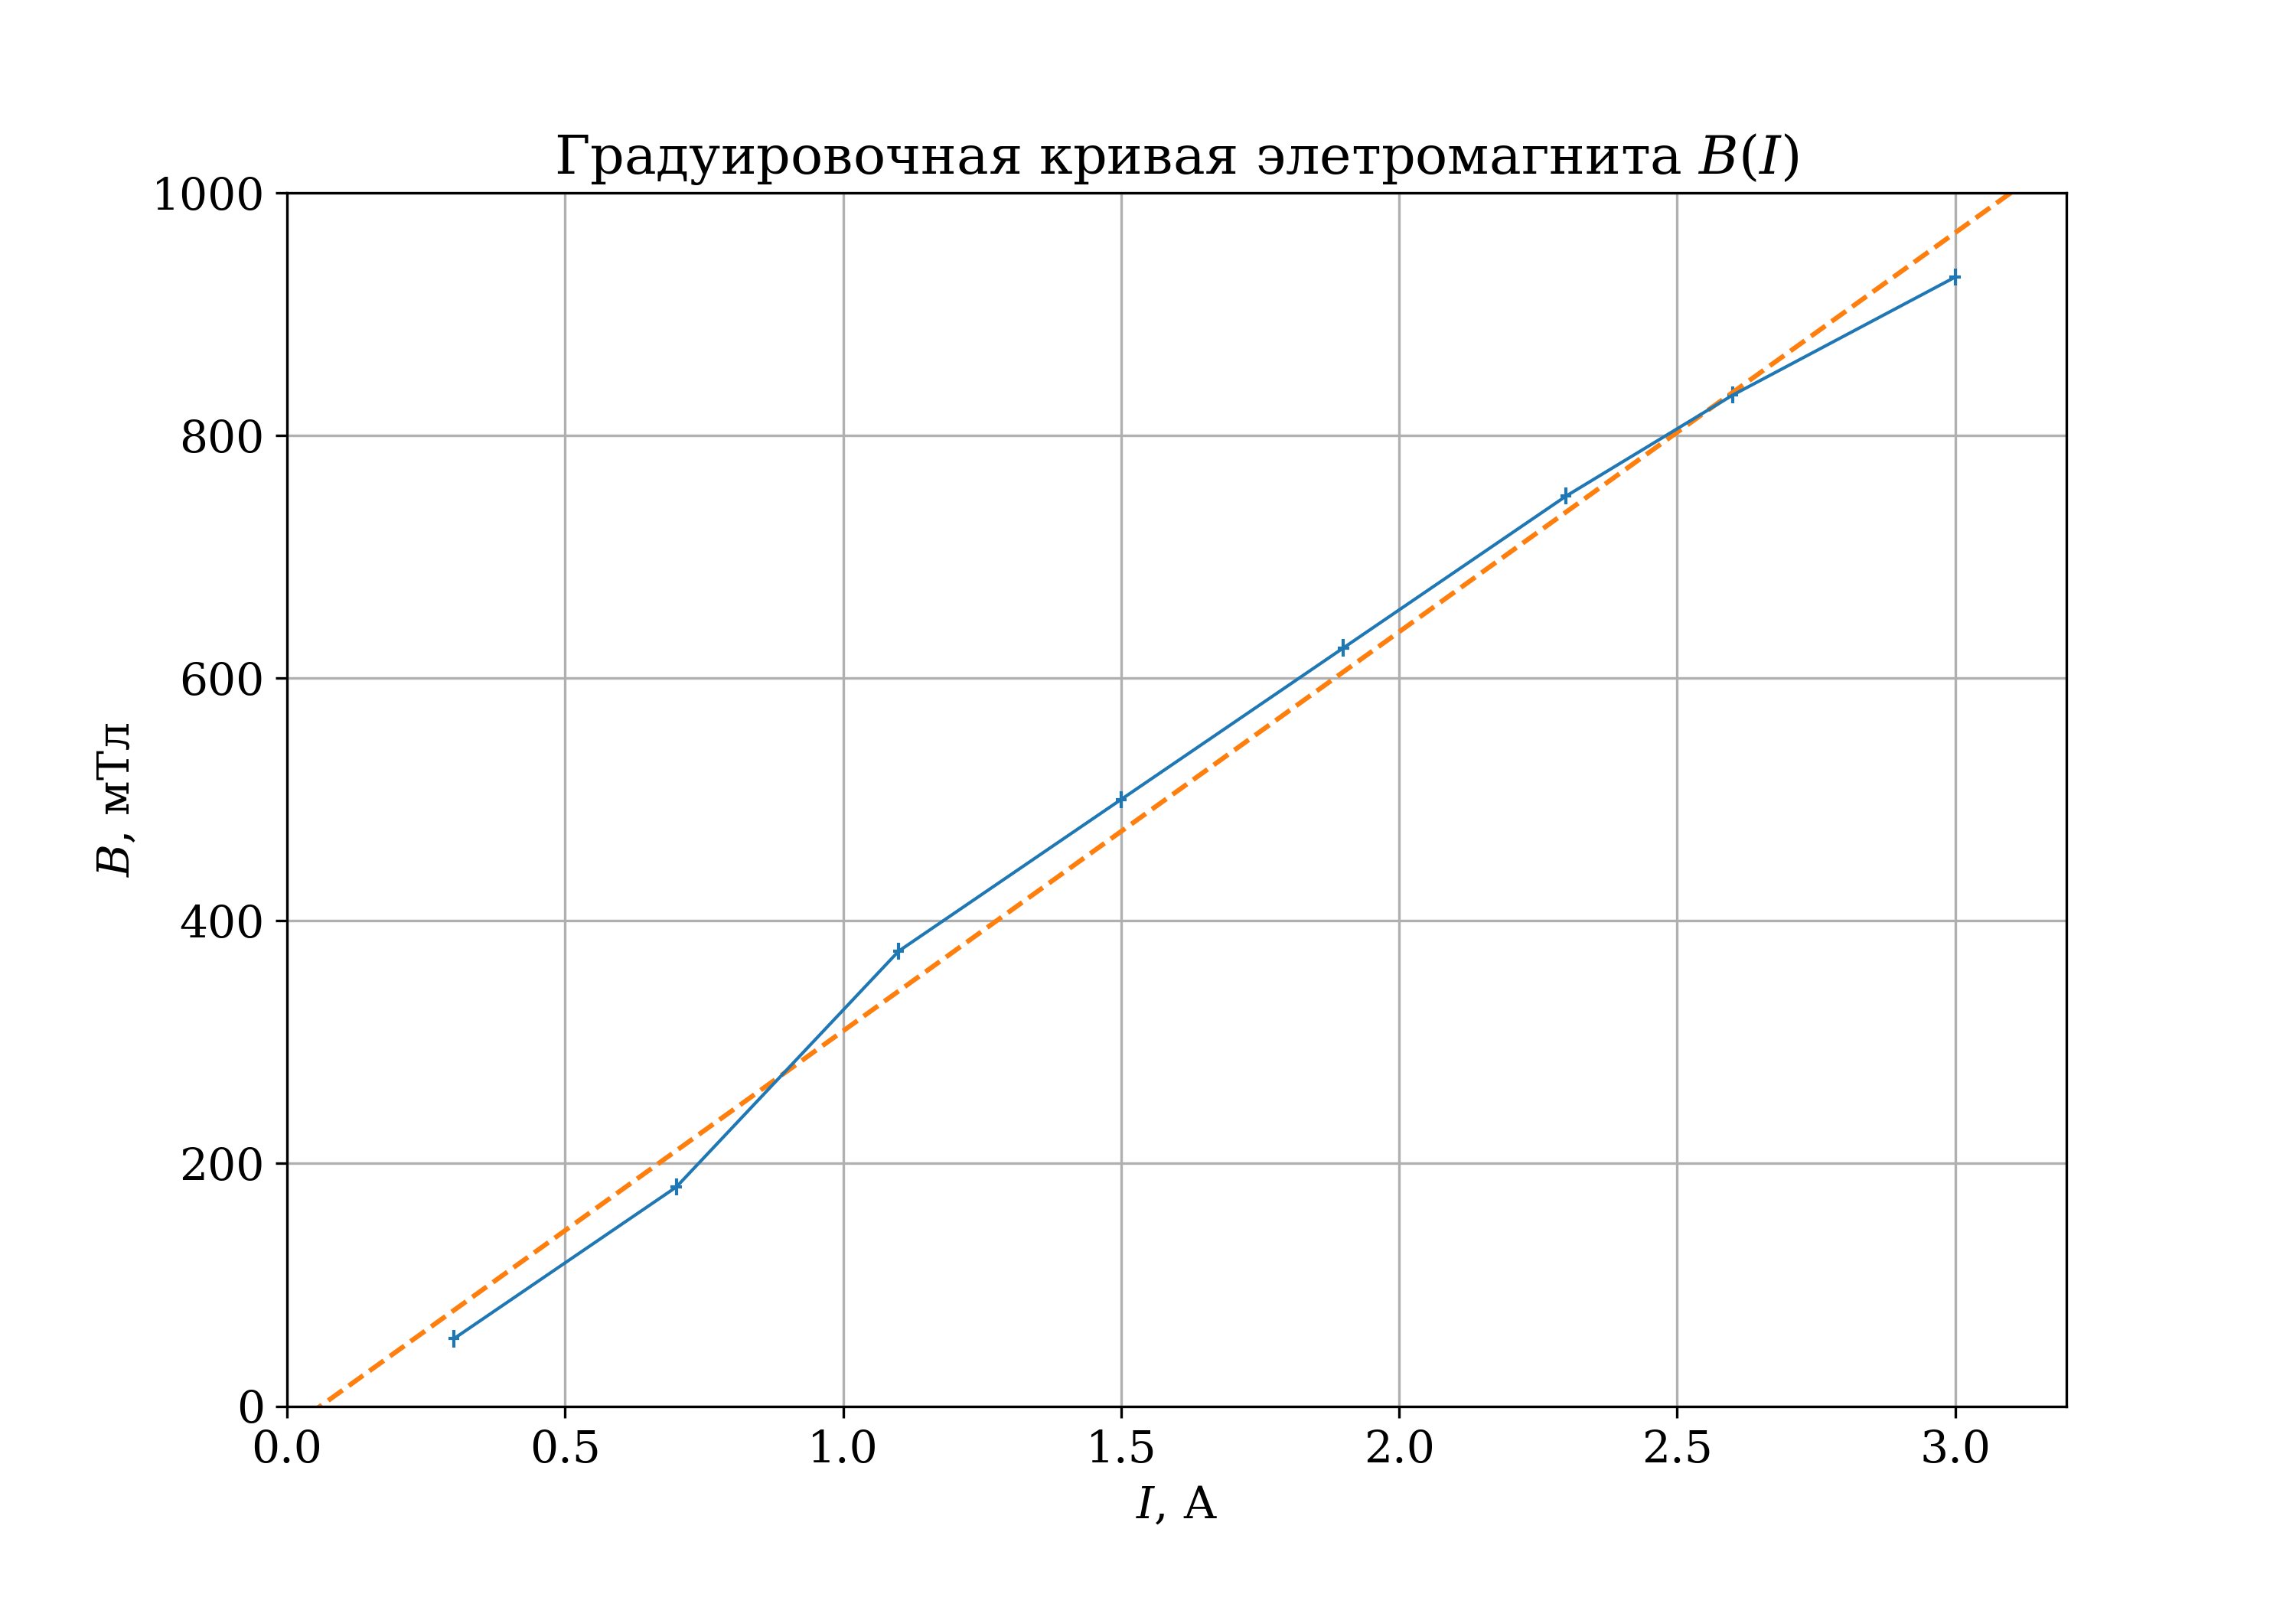
\includegraphics[width=\linewidth]{grad_plot.png}
\caption{График градуировочной кривой}
\label{fig:grad_plot}
\end{center}
\end{figure}

\subsection{Определение величины $\boldsymbol\chi$}

\paragraph{Измерим} перегрузку $\Delta P$ для образцов при различных значениях тока. Для 
этого сними показания весов $\Delta M$ при различных значениях $I$ и домножим на коэффициент $g$ ($P = mg$). Данные занесём в таблицу \ref{tab:measure}, значения снятые при увеличении и уменьшении силы тока помечены значками $\blacktriangle$ и $\blacktriangledown$ соответственно.

\begin{table}[h]
\begin{center}
\begin{tabular}{|c||c|c|c|c|c|c|c|c|c|}
\hline 
$I$ & 0 & 0.3 & 0.7 & 1.1 & 1.5 & 1.9 & 2.3 & 2.6 & 3.0 \\ 
\hline 
$\Delta M \blacktriangle$ Cu, мг & 0 & 0 & -2 & -4 & -6 & -11 & -14 & -17 & -21 \\ 
\hline 
$\Delta M \blacktriangledown$ Cu, мг & 0 & -2 & -3 & -6 & -9 & -12 & -16 & -18 & -- \\ 
\hline 
$\Delta P \blacktriangle$ Cu, мкН & 0 & 0 & -20 & -39 & -59 & -108 & -137 & -166 & -206 \\ 
\hline 
$\Delta P \blacktriangledown$ Cu, мкН & 0 & -20 & -30 & -59 & -88 & -118 & -157 & -176 & -- \\ 
\hline 
$\Delta M \blacktriangle$ Al, мг & 0 & 0 & 1 & 4 & 10 & 17 & 26 & 32 & 41 \\ 
\hline 
$\Delta M \blacktriangledown$ Al, мг & 2 & 2 & 2 & 7 & 11 & 19 & 27 & 34 & -- \\ 
\hline 
$\Delta P \blacktriangle$ Al, мкН & 0 & 0 & 10 & 39 & 98 & 166 & 255 & 314 & 402 \\ 
\hline 
$\Delta P \blacktriangledown$ Al, мкН & 20 & 20 & 20 & 69 & 108 & 186 & 265 & 333 & -- \\ 
\hline 
$\Delta M \blacktriangle$ C, мг & 0 & 8 & 24 & 37 & 39 & 39 & 34 & 28 & 10 \\ 
\hline 
$\Delta M \blacktriangledown$ C, мг & 8 & 17 & 33 & 46 & 46 & 46 & 37 & 26 & -- \\ 
\hline 
$\Delta P \blacktriangle$ C, мкН & 0 & 78 & 235 & 363 & 382 & 382 & 333 & 274 & 98 \\ 
\hline 
$\Delta P \blacktriangledown$ C, мкН & 78 & 167 & 323 & 451 & 451 & 451 & 363 & 255 & -- \\ 
\hline 
\end{tabular} 
\caption{Снятые экспериментальные данные}
\label{tab:measure}
\end{center}
\end{table}

\paragraph{Отметим} измеренные значения на графике и проведём аппроксимирующие кривые пользуясь методом наименьших квадратов (рис. \ref{plot_cu}, \ref{plot_al}, \ref{plot_c}).

\begin{figure}
\begin{center}
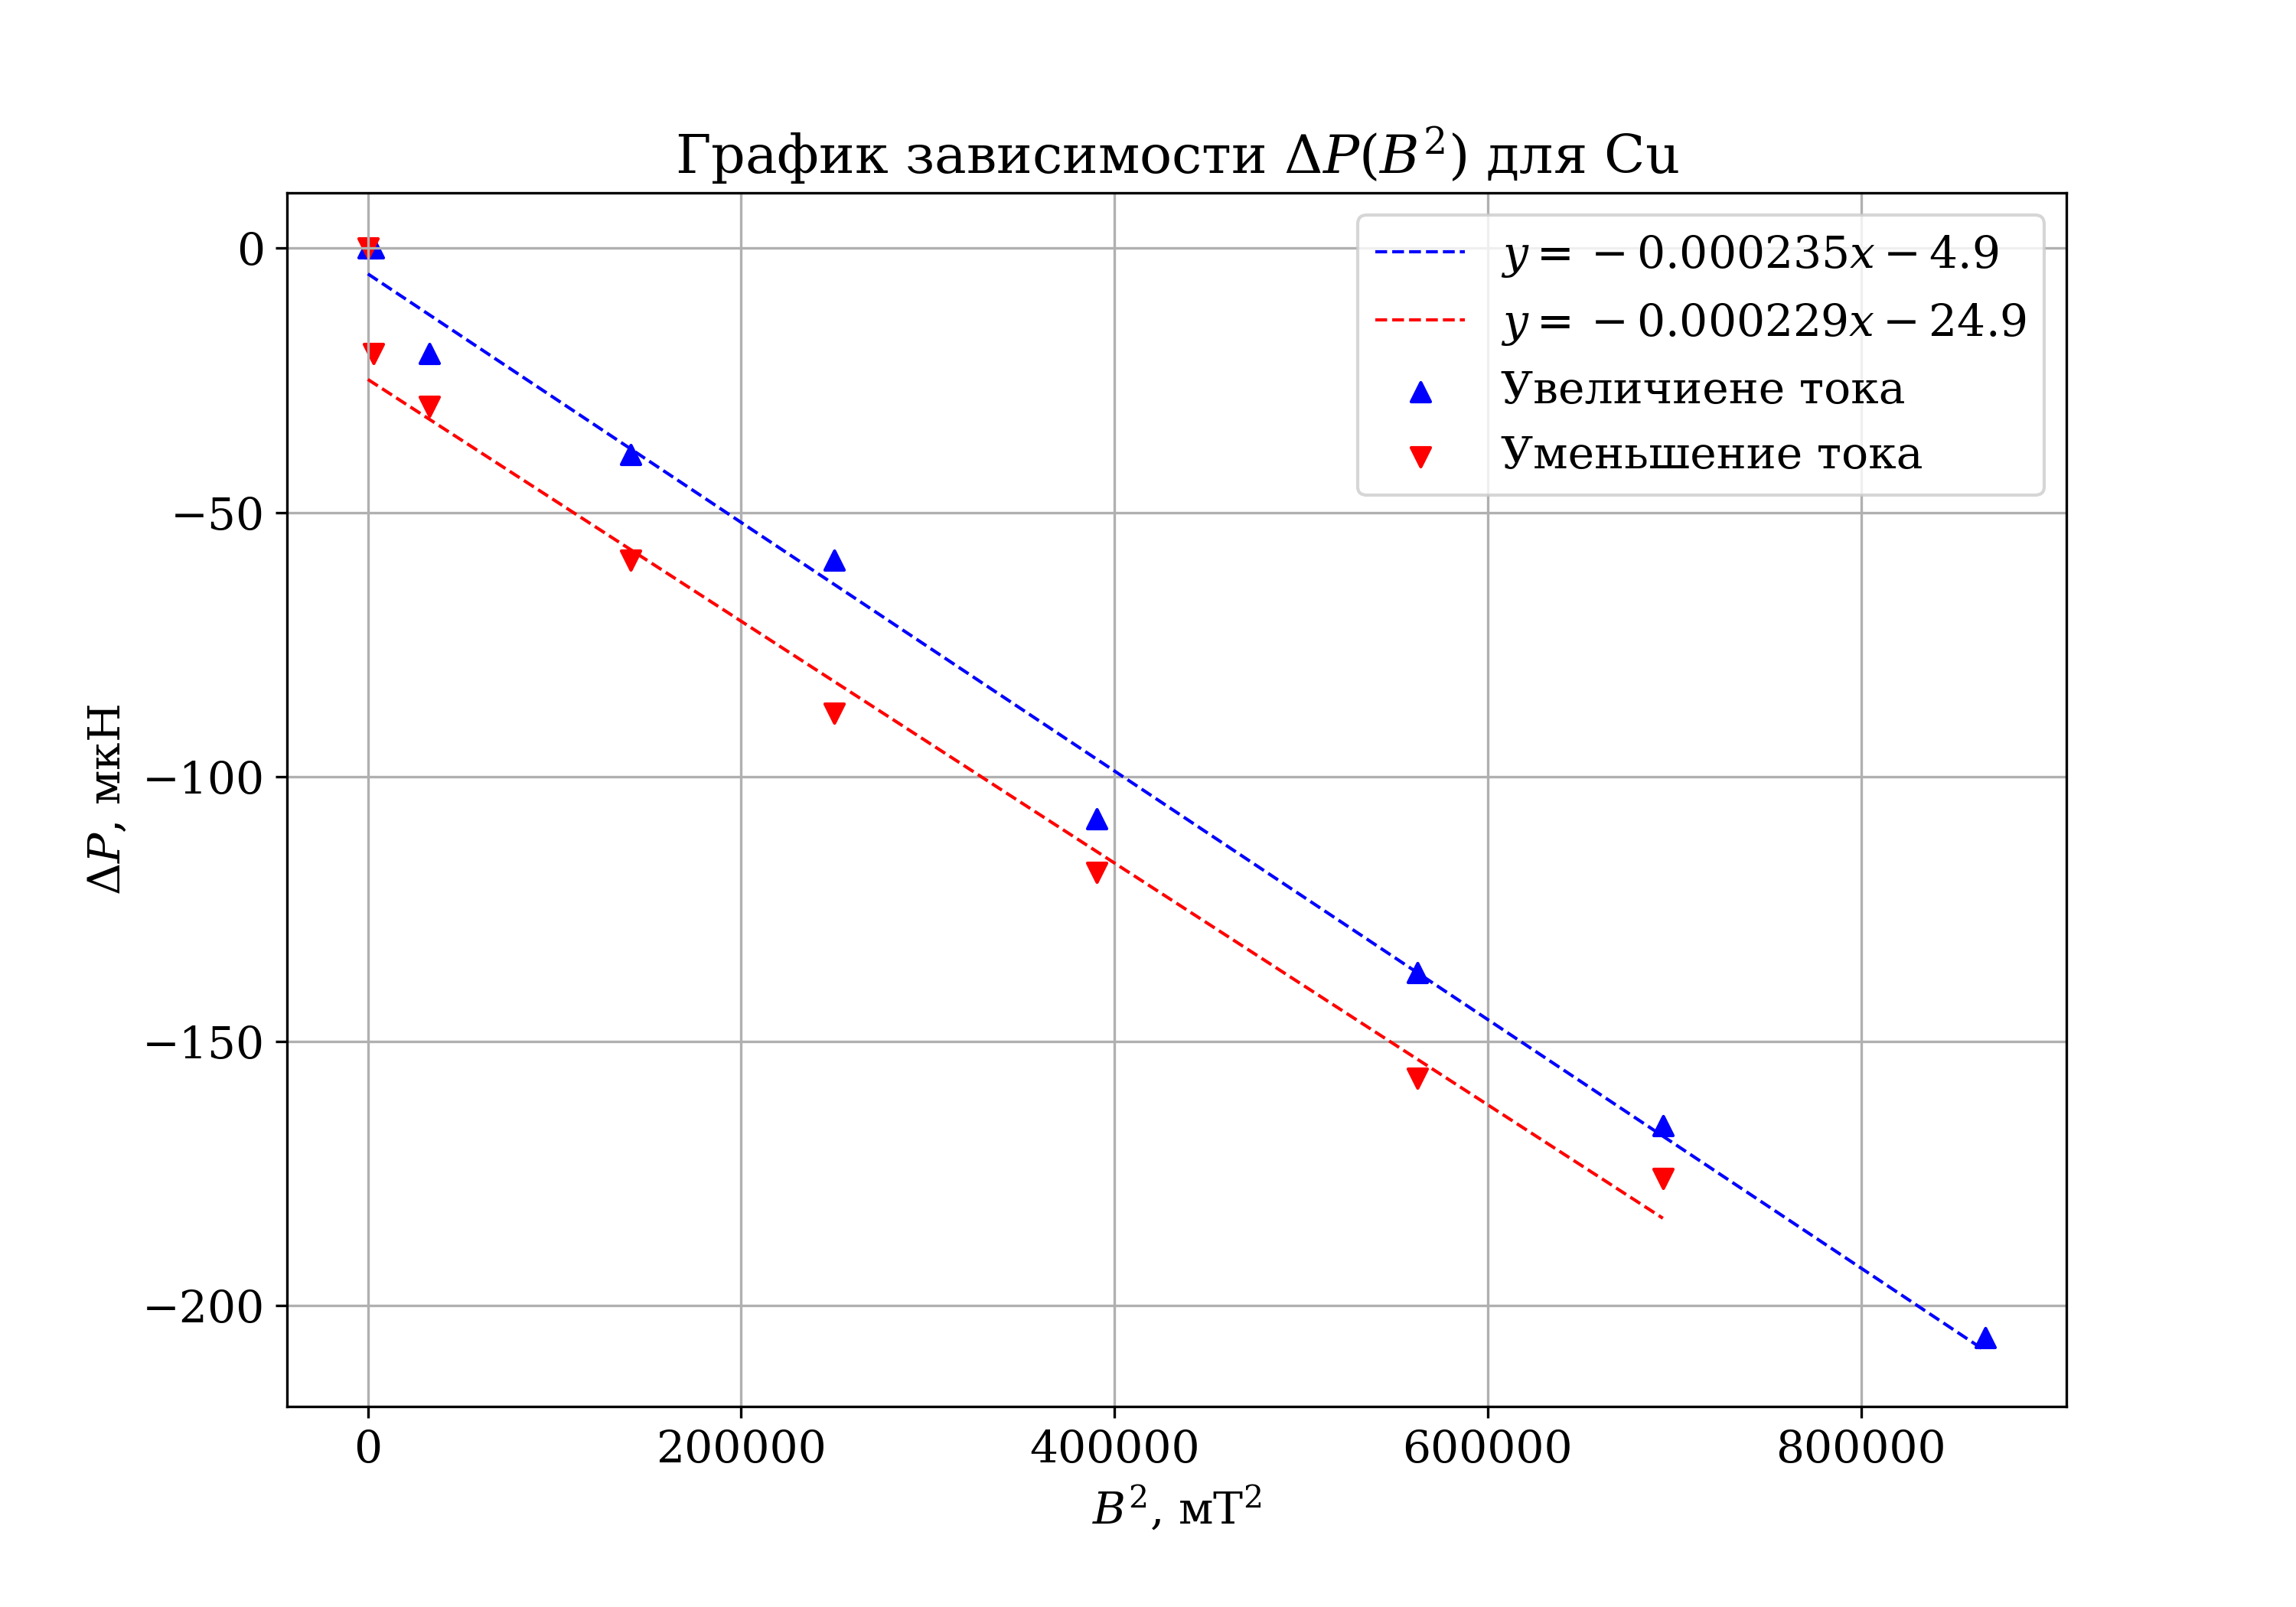
\includegraphics[width=\linewidth]{plot_cu.png}
\caption{График для Cu}
\label{plot_cu}
\end{center}
\end{figure}

\begin{figure}
\begin{center}
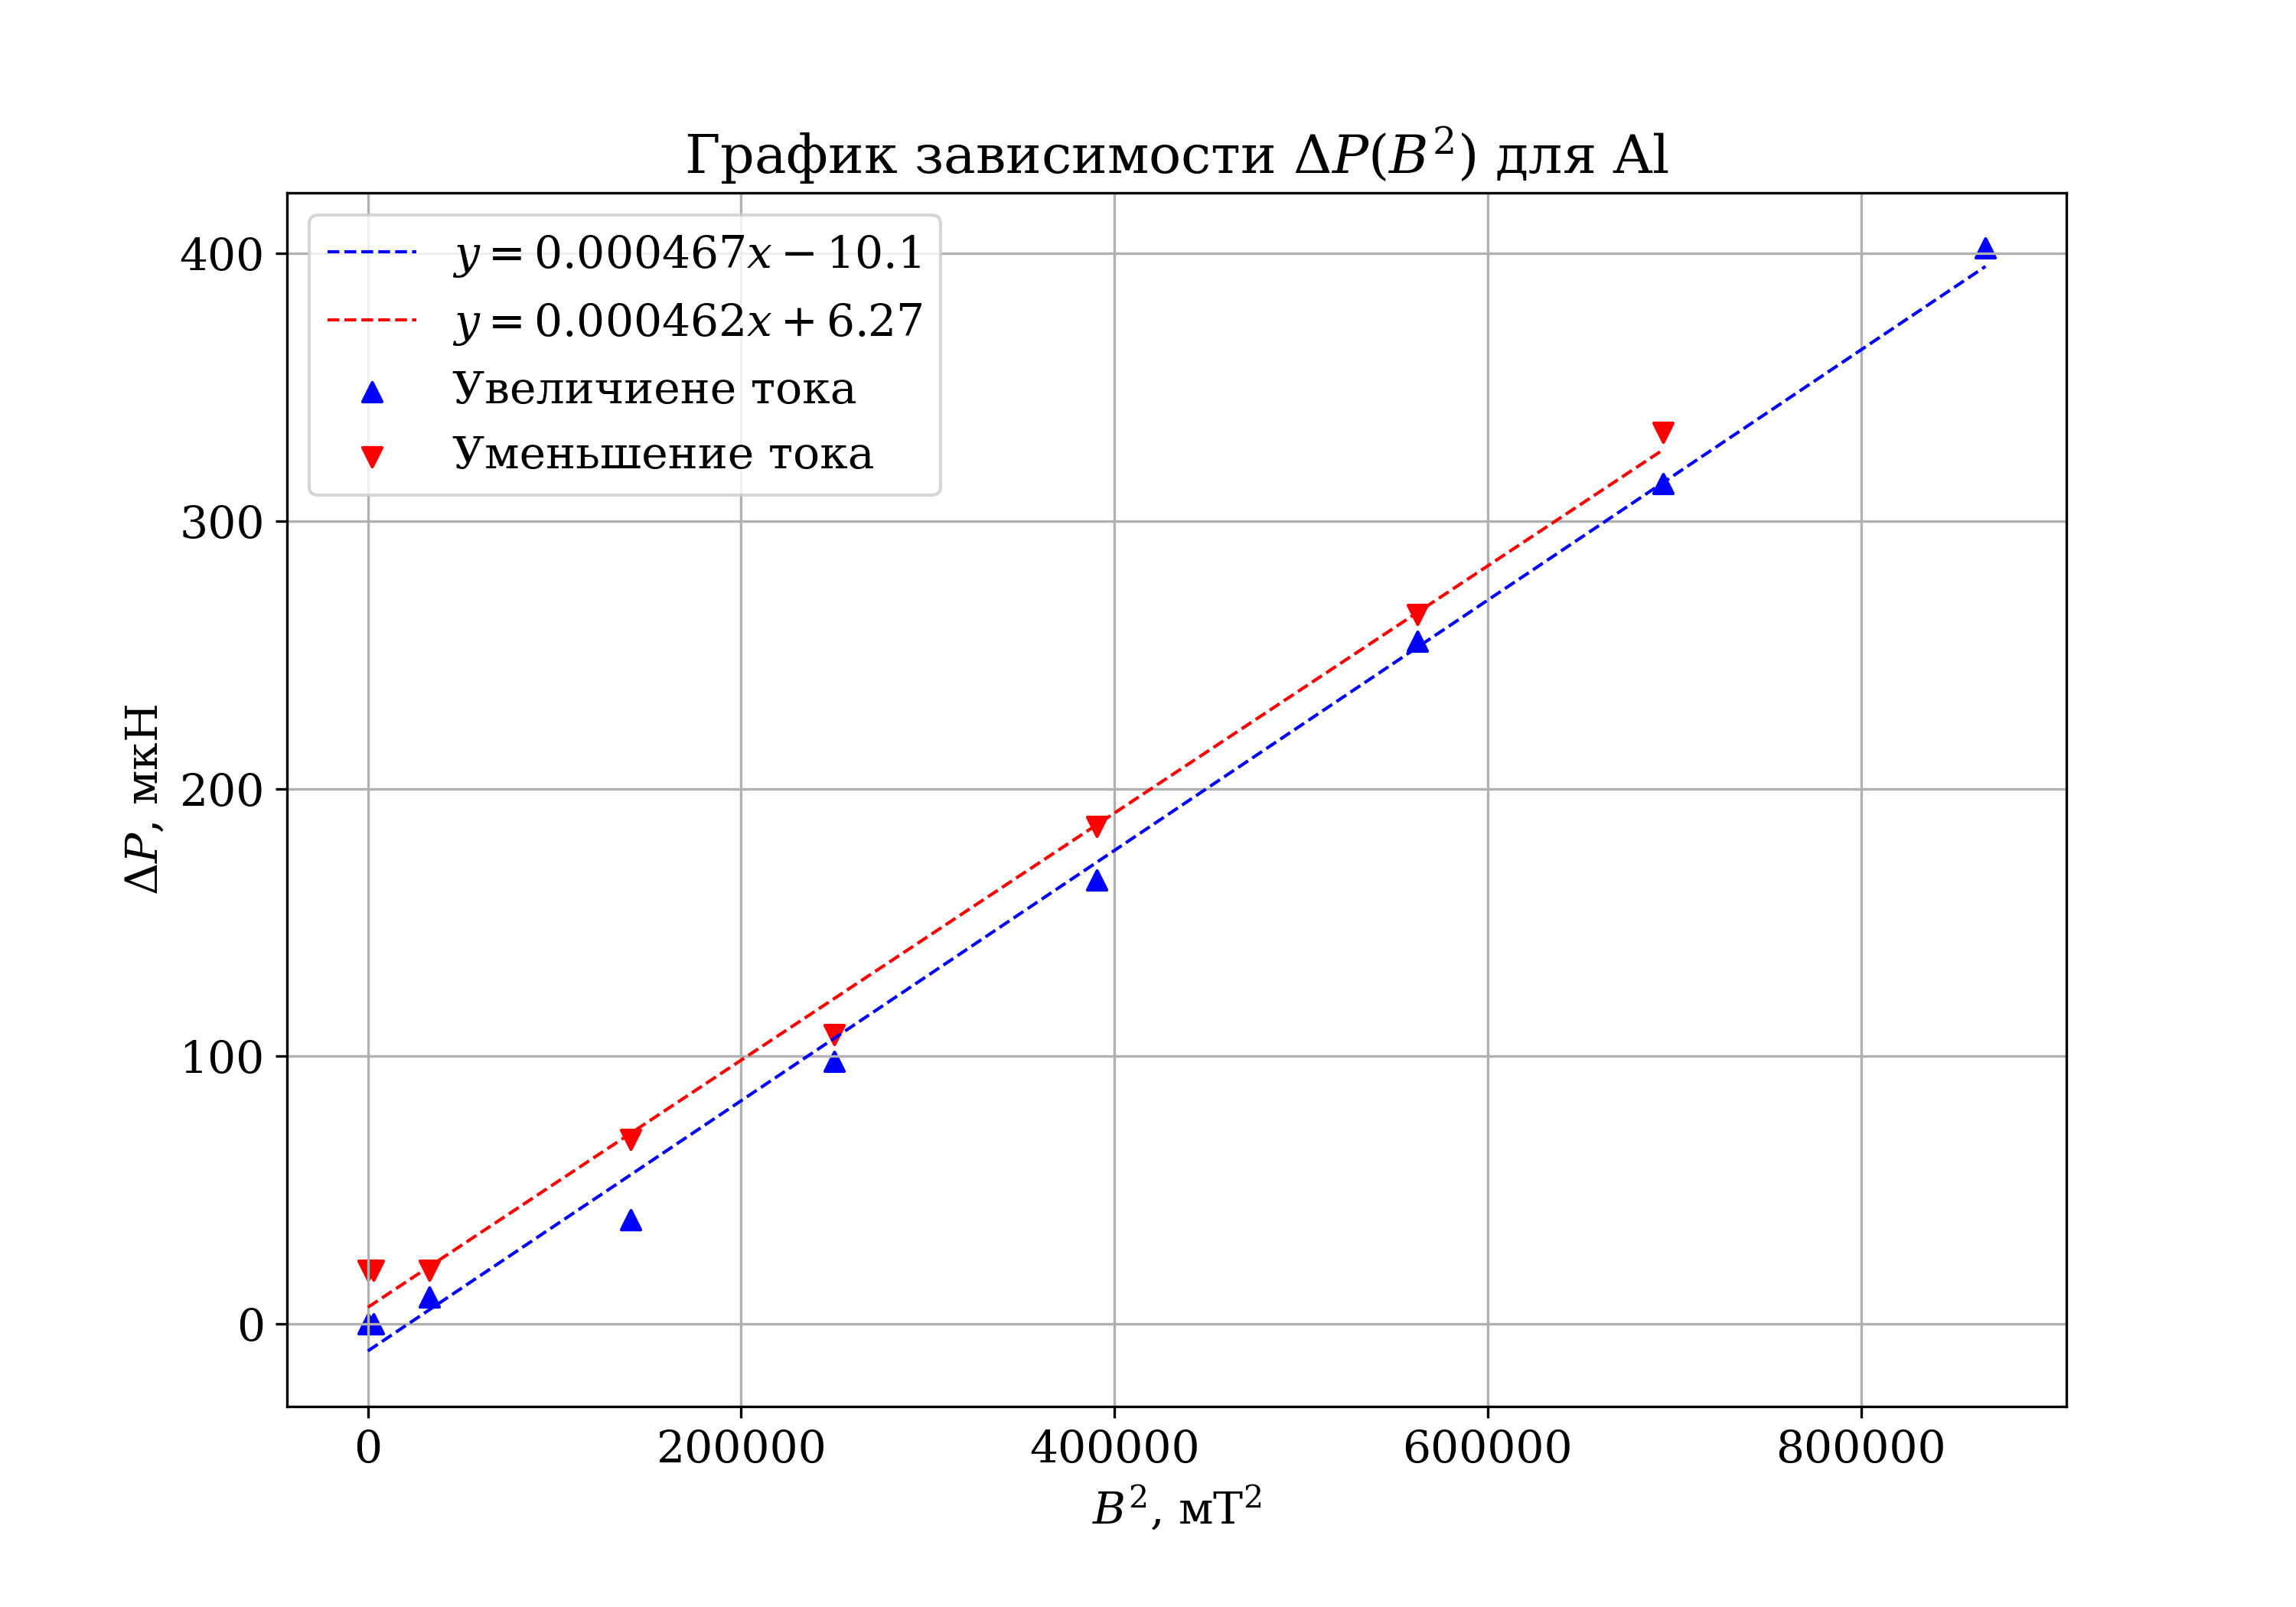
\includegraphics[width=\linewidth]{plot_al.png}
\caption{График для Al}
\label{plot_al}
\end{center}
\end{figure}

\begin{figure}
\begin{center}
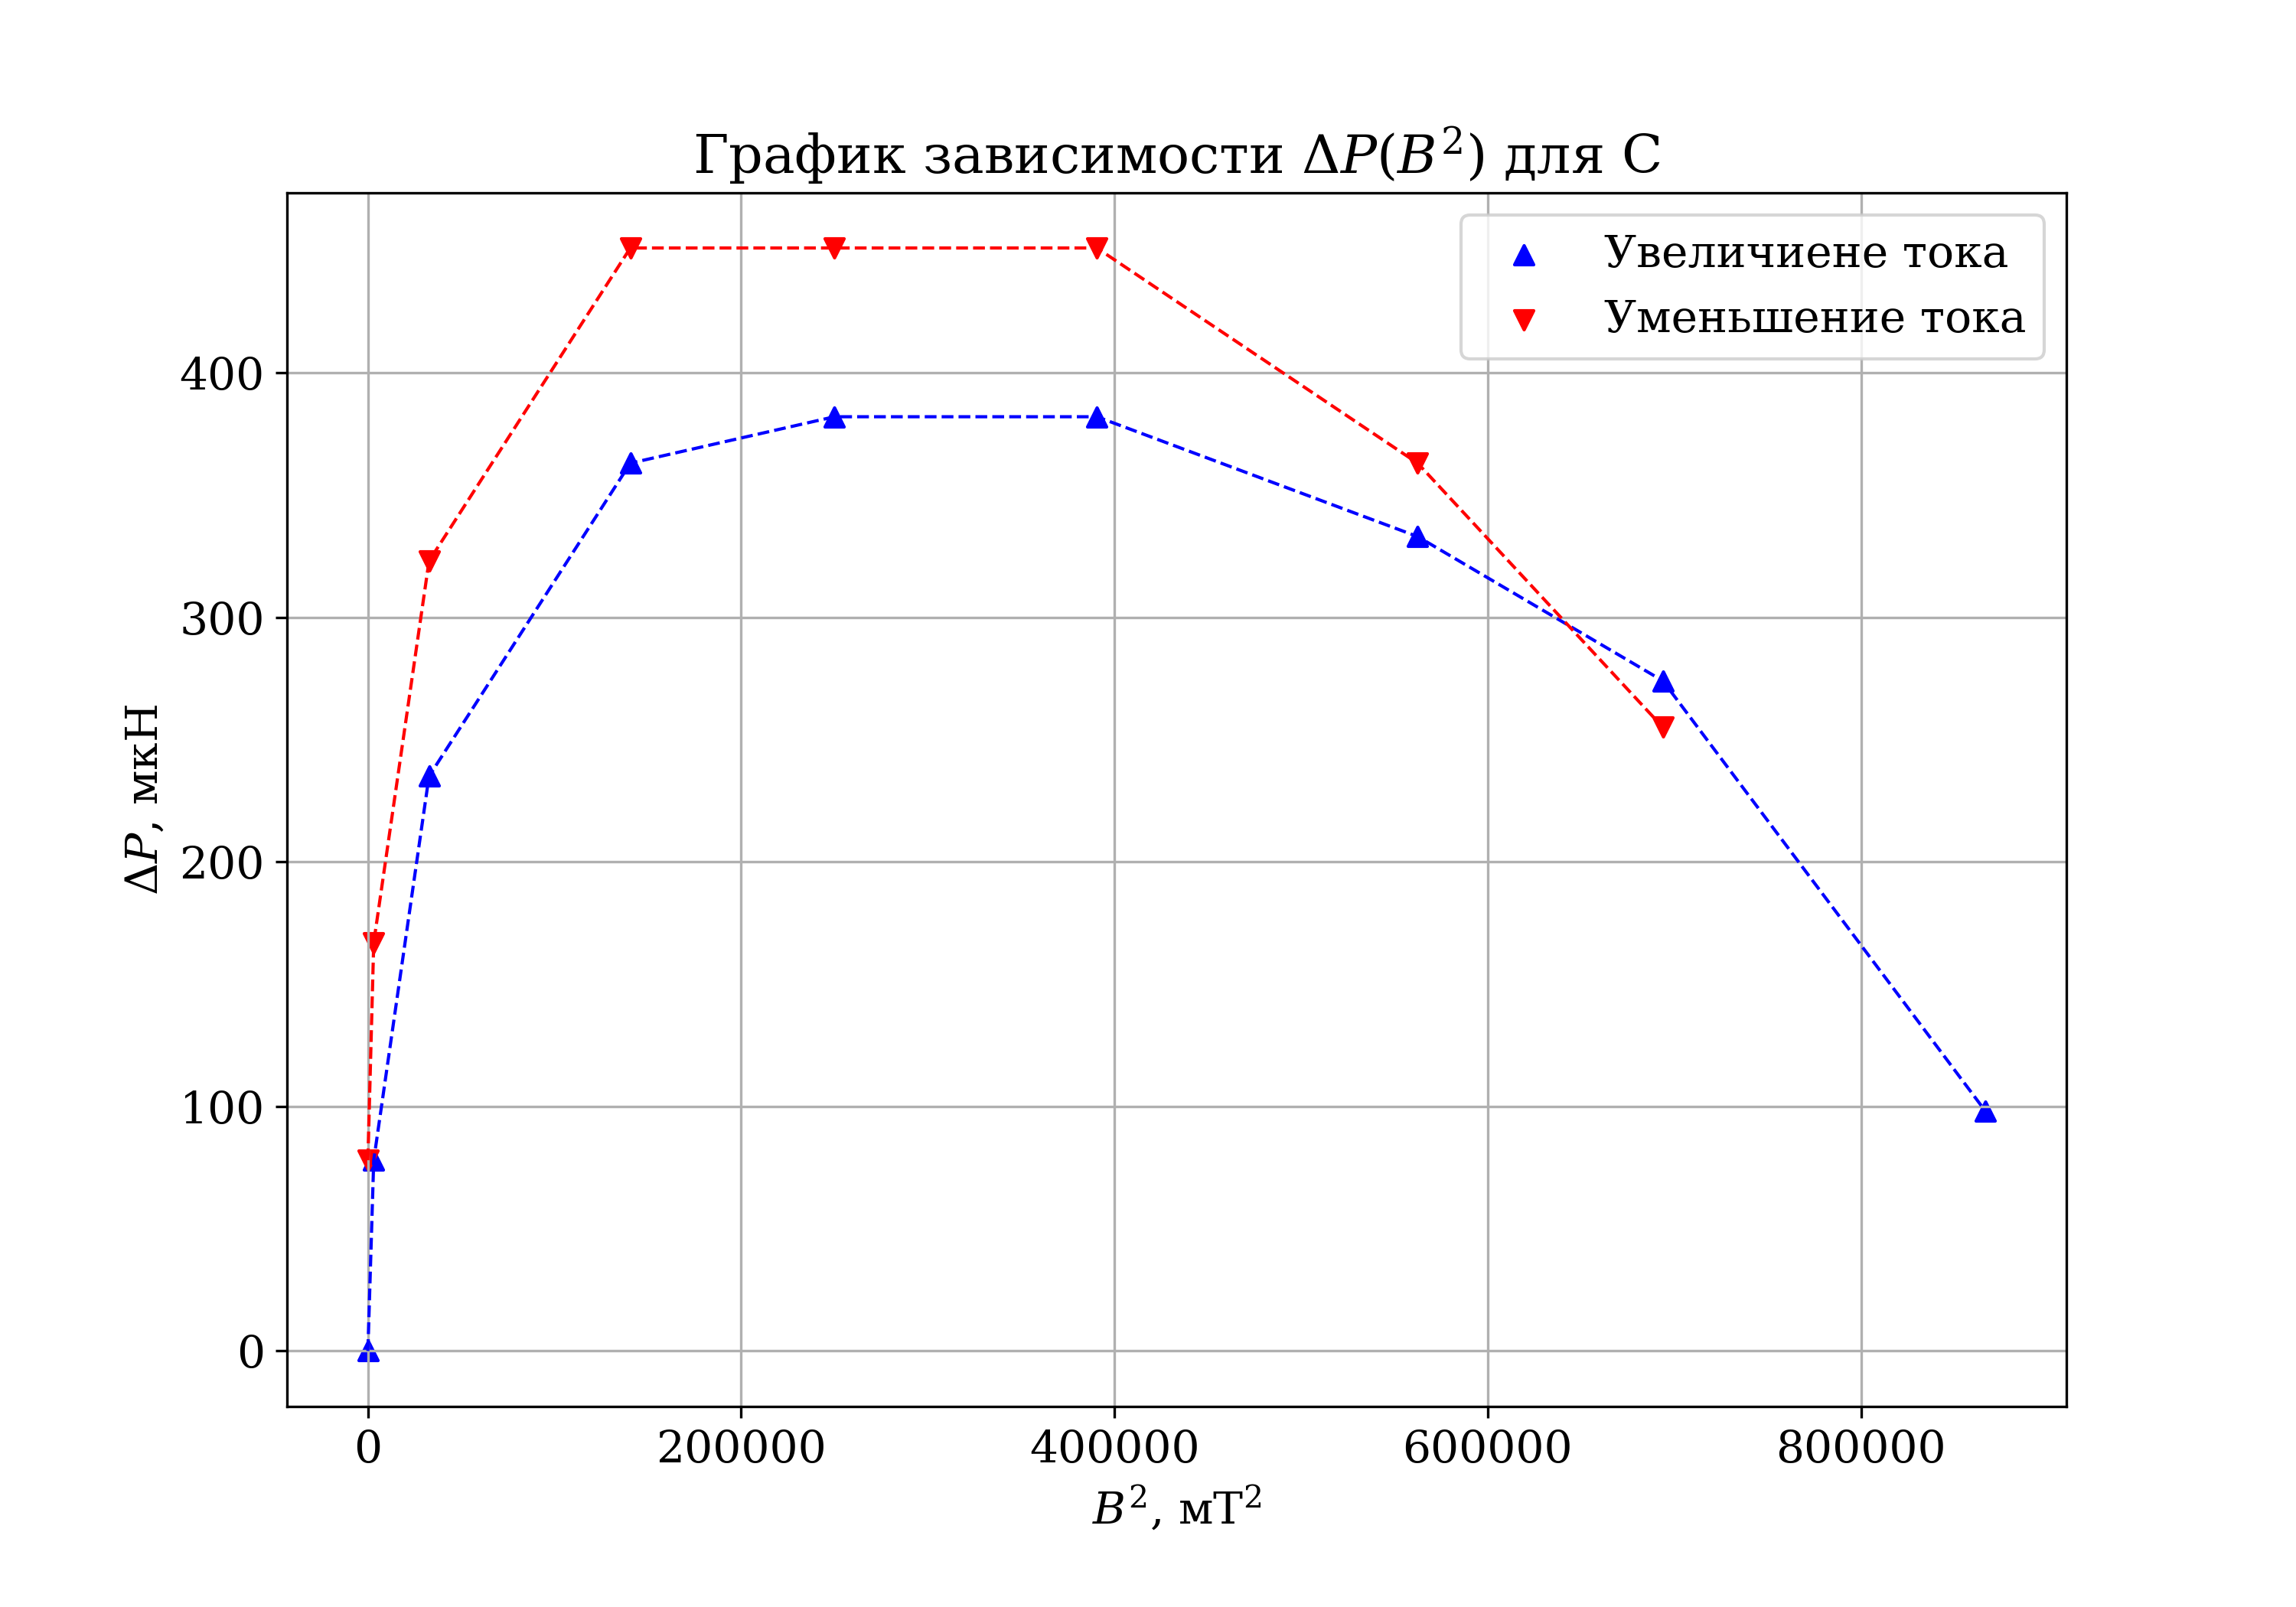
\includegraphics[width=\linewidth]{plot_c.png}
\caption{График для C}
\label{plot_c}
\end{center}
\end{figure}

\paragraph{Получим} значения $\chi$ и погрешности $\sigma_\chi$ пользуясь формулой:
\[ \Delta P = \frac{\chi s}{2 \mu_0} B^2 = \alpha B^2 \Rightarrow \chi = \frac{2 \alpha \mu_0}{s} \Rightarrow \chi_\text{уд} = \frac{2 \alpha \mu_0}{s \rho} ,\]
где $\alpha$ -- коэффициент наклона аппроксимирующей прямой рассчитанной пользуясь методом наименьших квадратов, $s$ -- площадь сечения образца $s = \pi d^2 / 4 = \pi / 4$ см$^2$. 

Для \textbf{Cu} получаем:

\[ \alpha_\blacktriangle = -(235 \pm 6) \cdot 10^{-6} \; \frac{\text{мкН}}{\text{мТл}^2} =-(235 \pm 6) \cdot 10^{-6} \; \frac{\text{Н}}{\text{Тл}^2}, \]

\[ \alpha_\blacktriangledown = -(229 \pm 7) \cdot 10^{-6} \; \frac{\text{мкН}}{\text{мТл}^2} =-(229 \pm 7) \cdot 10^{-6} \; \frac{\text{Н}}{\text{Тл}^2}. \]

Берём среднее $\alpha_\textbf{Cu} = - (2.3 \pm 0.1) \cdot 10^{-4}$ Н/Тл$^2$, из чего получаем: 
\[\chi_\text{Cu} = - \frac{8 \pi \cdot 10^{-7} \cdot (2.3 \pm 0.1) \cdot 10^{-4}}{\pi \cdot 0.005^2 \cdot 8960} = - (8.2 \pm 0.4) \cdot 10^{-10} \;\frac{\text{м}^3}{\text{кг}}.\] 

Для \textbf{Al} получаем:

\[ \alpha_\blacktriangle = (467 \pm 9) \cdot 10^{-6} \; \frac{\text{мН}}{\text{мТл}^2} = (467 \pm 9) \cdot 10^{-6} \; \frac{\text{Н}}{\text{Тл}^2}, \]

\[ \alpha_\blacktriangledown = (462 \pm 11) \cdot 10^{-6} \; \frac{\text{мН}}{\text{мТл}^2} = (462 \pm 11) \cdot 10^{-6} \; \frac{\text{Н}}{\text{Тл}^2}. \]

Берём среднее $\alpha_\textbf{Al} = (4.6 \pm 0.2) \cdot 10^{-4}$ Н/Т$^2$, из чего получаем: 
\[\chi_\text{Al} = \frac{8 \pi \cdot 10^{-7} \cdot (4.6 \pm 0.2) \cdot 10^{-4}}{\pi \cdot 0.005^2 \cdot 2700} = (5.6 \pm 0.3) \cdot 10^{-9}\;\frac{\text{м}^3}{\text{кг}}.\] 

Для \textbf{C} график получился нелинейным, что может быть связано с наличием в стержне из графита ферромагнитных примесей.

\medskip\hrule\medskip


\section{Выводы}

Мы провели исследование поведения диа- и парамагнетиков в магнитном поле и показали, что выполняются зависимости лежащие в основе метода Гюи. 

Мы нашли значения для удельной магнитной восприимчивости меди и алюминия, и получили значения:

\[\chi_\text{Cu} = - (8.2 \pm 0.4) \cdot 10^{-10}\;\frac{\text{м}^3}{\text{кг}}, \;\;\; \chi_\text{Al} = (5.6 \pm 0.3) \cdot 10^{-9}\;\frac{\text{м}^3}{\text{кг}}.\]

Табличные значения: 
\[\chi_\text{Cu, табл.} = - 8.6 \cdot 10^{-10}\;\frac{\text{м}^3}{\text{кг}}, \;\;\; \chi_\text{Al, табл.} = 6.1 \cdot 10^{-9}\;\frac{\text{м}^3}{\text{кг}}.\]

Видим, что измеренные значения достаточно близки 

\medskip\hrule\medskip

\end{document}
